%!Tex Root = ../main.tex
% ./Packete.tex
% ./Design.tex
% ./Deklarationen.tex
% ./Vorbereitung.tex
% ./Aufgabe1.tex
% ./Aufgabe2.tex
% ./Aufgabe3.tex
% ./Aufgabe4.tex

\section{Appendix}

\begin{frame}[allowframebreaks]{Appendix}{Zahlendarstellungen zur Basis b - Stellenwertsysteme}
  \begin{itemize}
    \item \alert{Zahlensytem} $S = (b, Z, \delta)$
    \begin{itemize}
  \item Zahlensystem wird durch Anhängen der \alert{Basis als Index} an die Ziffernfolge ${d_{n-1}\ldots d_{0}}_b$ vermittelt
      \item \alert{Basis} $b\in\mathbb{N}, b\rangle 1$ mit welcher für jede \alert{Stelle} $i$ der \alert{Stellenwert} $b^i$ berechnet wird
      \item \alert{Ziffernmenge} $Z$
      \item \alert{Ziffernwertigkeit} $\delta$ ordnet jeder \alert{Ziffer} bzw. Symbol ihre \alert{Wertigkeit} zu
% $(z_i)_{i=0,\ldots,n}$
% $z\ =\ z_{n-1}\ldots z_{0}$
    \end{itemize}
    \begin{Sidenote}
      \begin{itemize}
        \item bei der $n$-stelligen Binärdarstellung einer Zahl werden dem \alert{LSB} und \alert{MSB} jeweils die Stellenwerte $b^0$ und $b^{n-1}$ zugeordnet
        \item Im \alert{Binärsystem / Dualsystem} werden den beiden Ziffern $0$ und $1$ jeweils die Wertigkeiten $0$ und $1$ zugeordnet
        \item Im \alert{Dezimalsystem} werden den zehn Ziffern $0, 1, 2, 3, 4, 5, 6, 7, 8$ und $9$ jeweils die Wertigkeiten $0$ bis $9$ in der konventionellen Reihenfolge zugeordnet
        \item Im \alert{Hexadezimalsystem} werden den sechzehn Ziffern $0, 1, 2, 3, 4, 5, 6, 7, 8, 9, A, B, C, D, E$ und $F$ jeweils die Werte der Dezimalzahlen von $0$ bis $15$ zugeordnet.
        \begin{itemize}
          \item \alert{Eselsbrücken:} \alert{C}wölf, \alert{D}reizehn, \alert{F}ünfzehn
        \end{itemize}
    \end{itemize}
\end{Sidenote}
    \item \alert{positiver Wert} $\displaystyle \langle d\rangle\ =\ \sum_{i=0}^{n-1} \delta(d_{i})\cdot b^{i}$ einer \alert{nicht-negativen Natürlichen Zahl}, wobei $d=d_{n-1}\ldots d_0$ mit $d_i\in Z$ eine \alert{Folge} von $n$ \alert{Ziffern} bzw. Symbolen ist
  \end{itemize}
\end{frame}

\begin{frame}[allowframebreaks]{Appendix}{Zahlendarstellung zur Basis b - Stellenwertsysteme\vspace{0.5cm}}
  \begin{itemize}
    \item \alert{positiver Wert} $\displaystyle \langle d\rangle=\sum_{i=-k}^{n-1}\delta(d_{i})\cdot b^{i}$ einer \alert{nicht-negativen Festkommazahl}, wobei $d=d_{n-1}\ldots d_0\ldots d_{-k}$ mit $d_i\in Z$
    \begin{itemize}
      \item \alert{die Anzahl der Nachkommastellen ist fest:} $\langle d_{n-1}\ldots d_0 d_{-1}\ldots d_{-k}\rangle \cdot 2^{-k} = \langle d_{n-1}\ldots d_0\textcolor{PrimaryColor}{\bm .}d_{-1}\ldots d_{-k}\rangle$
      \item Beispiel 3-Bit Festkommazahlen mit $n=1$ und $k=2$:
        \begin{table}
          \raggedright
          \begin{tblr}{
              cells = {c, BoxColor},
              column{1} = {PrimaryColor,fg=white},
            }
            $d$                & 0.00 & 0.01 & 0.10 & 0.11 & 1.00 & 1.01 & 1.10 & 1.11 \\
            $\langle d\rangle$ & 0.0  & 0.25 & 0.5  & 0.75 & 1.0  & 1.25 & 1.5  & 1.75 \\
          \end{tblr}
        \end{table}
    \end{itemize}
  \end{itemize}
  \begin{figure}
    \begin{subfigure}{0.4\textwidth}
      \centering
      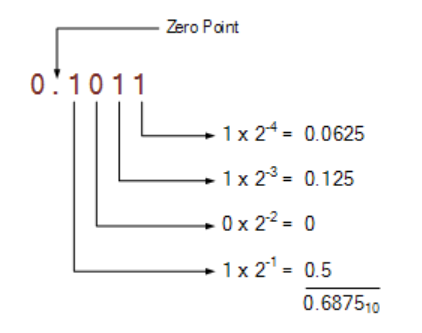
\includegraphics[width=0.8\linewidth]{figures/binary_fraction}
      \caption{Binärerbrüche}
      \label{fig:binaryfraction}
    \end{subfigure}
    \begin{subfigure}{0.4\textwidth}
      \centering
      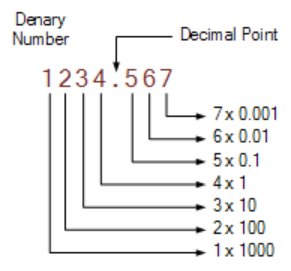
\includegraphics[width=0.6\linewidth]{figures/decimal_fraction}
      \caption{Dezimalbrüche}
      \label{fig:decimalfraction}
    \end{subfigure}
  \end{figure}
  \begin{itemize}
    \item Darstellung \alert{negativer Festkommazahlen}, wobei $d=d_{n}d_{n-1}\ldots d_0\ldots d_{-k}$ mit $\forall i\langle n:d_i\in Z$ und $d_n\in\{0, 1\}$:
    \begin{itemize}
      \item \alert{potentiell negativer Wert} $\displaystyle[d]_{BV} = (-1)^{d_n}\sum_{i=0}^{n-1}\delta(d_i)2^i$ in \alert{Darstellung durch Betrag und Vorzeichen}
      \begin{itemize}
        \item Beispiel 3-Bit Festkommazahlen mit Vorzeichenbit, $n=1$ und $k=1$:
          \begin{table}
            \raggedright
            \begin{tblr}{
                cells = {c, BoxColor},
                column{1} = {PrimaryColor,fg=white},
              }
              $d$        &  11.1  & 11.0 & 10.1 & 10.0 & 00.0 & 00.1 & 01.0 & 01.1 \\
              $[d]_{BV}$ & -1.5 & -1.0 & -0.5 & 0.0 & 0.0   & 0.5 & 1.0  & 1.5 \\
            \end{tblr}
          \end{table}
      \end{itemize}
    \item \alert{potentiell negativer Wert} $\displaystyle[d]_{1} = \sum_{i=0}^{n-1}\delta(d_i) 2^i - \delta(d_n)(2^n-2^{-k})$ in \alert{Einerkomplement-Darstellung}
      \begin{itemize}
        \item Beispiel 3-Bit Festkommazahlen mit Vorzeichenbit, $n=1$ und $k=1$:
          \begin{table}
            \raggedright
            \begin{tblr}{
                cells = {c, BoxColor},
                column{1} = {PrimaryColor,fg=white},
              }
              $d$                & 10.0 & 10.1 & 11.0 & 11.1 & 00.0 & 00.1 & 01.0 & 01.1 \\
              $[d]_1$ & -1.5  & -1.0 & -0.5  & 0.0 & 0.0  & 0.5 & 1.0  & 1.5 \\
            \end{tblr}
          \end{table}
      \end{itemize}
      \begin{itemize}
        \item im Negativen hat eine Folge mit mehr $1$en anders als im Positiven betragsmäßig eine kleineren Wert, denn umso mehr $1$en da sind, umso größer wird die Summe $\sum_{i=0}^{n-1}\delta(d_i)2^i$ und umso mehr kann von der subtrahierten größten positiven Zahl $2^n-1$ ausgeglichen werden
        \item um den Wert einer negativen Dezimalzahl binär darzustellen gibt es 2 Methoden
          \begin{description}[abc]
            \item[1.] mit größtmöglichen positven Zahl anfangen $-(2^n-1)$ und überlegen, welche $2$er Potenzen (Stellenwerte) man draufaddieren muss, um die gewünschte Zahl zu erhalten und an den entsprechenden Bits, die diesen $2$er Potenzen entsprechen $1$en setzen
            \item[2.] die passende Ziffernfolge wie gewohnt erstellen, aber mit vertauschten $1$en und $0$en und das Vorzeichenbit ist eine $1$
          \end{description}
      \end{itemize}
      \item \alert{potentiell negativer Wert} $\displaystyle[d]_{2} = \sum_{i=0}^{n-1}\delta(d_i)2^i - \delta(d_n)2^n$ in \alert{Zweierkomplement-Darstellung}
      \begin{itemize}
        \item Beispiel 3-Bit Festkommazahlen mit Vorzeichenbit, $n=1$ und $k=1$:
          \begin{table}
            \raggedright
            \begin{tblr}{
                cells = {c, BoxColor},
                column{1} = {PrimaryColor,fg=white},
              }
              $d$                & 10.0 & 10.1 & 11.0 & 11.1 & 00.0 & 00.1 & 01.0 & 01.1 \\
              $[d]_2$ & -2  & -1.5 & -1.0  & -0.5 & 0.0  & 0.5 & 1.0  & 1.5 \\
            \end{tblr}
          \end{table}
      \end{itemize}
      \begin{itemize}
        \item genauso wie beim Einerkomplment bedeuten mehr $1$en im Negativen einen betragsmäßig kleineren Wert
        \item um den Wert einer negativen Dezimalzahl binär darzustellen gibt es 2 Methoden
          \begin{description}[abc]
            \item[1.] mit der größtmöglichen positven Zahl + kleinmöglichen positven Zahl ungleich $0$ anfangen $-(2^n)$ und überlegen, welche $2$er Potenzen (Stellenwerte) man draufaddieren muss, um die gewünschte Zahl zu erhalten und an den entsprechenden Bits, die diesen $2$er Potenzen entsprechen $1$en setzen
            \item[2.] die passende Ziffernfolge wie gewohnt erstellen, aber die kleinstmögliche positve Zahl ungleich $0$ wird als Startwert genommen und die $1$en und $0$en sind vertauscht, sowie das Vorzeichenbit ist eine $1$
          \end{description}
        \item wenn man die kleinste negative Zahl komplementiert: $[10.0]_2' = [01.1]_1 + 1 = [10.0]_2$, dann erhält man erneut die kleinste negative Zahl. Das passt auch ganz gut, da die kleinste negative Zahl im Zweierkomplement keine komplementäre positive Zahl hat
      \end{itemize}
    \end{itemize}
  % \item Darstellung \alert{negativer Gleitkommazahlen}, wobei $d=\;$\partition[equal height group = fp, borderline west={0.25mm}{0mm}{black}]{sign bit}\partition[equal height group = fp, borderline east={0.25mm}{0mm}{black}, borderline west={0.25mm}{0mm}{black}]{exponent}\partition[equal height group = fp, borderline east={0.25mm}{0mm}{black}]{fraction/mantissa} mit exponent, fraction bits und sign bit aus $\{0, 1\}$:
  \item Darstellung \alert{negativer Gleitkommazahlen}, wobei $\underbrace{d_n}_{sign} \underbrace{d_{n-1} \ldots d_0}_{exponent} \underbrace{d_{-1}\ldots d_{-k}}_{fraction / mantissa}$ mit exponent, fraction bits und sign bit aus $\{0, 1\}$:
  \begin{itemize}
      \item \alert{varierende Anzahl von Nachkommastellen} im Gegensatz zu Festkommazahlen
      \item \alert{Normalisierte Zahlen:} $(-1)^{d_n} \cdot \langle 1 d_{-1}\ldots d_{-k}\rangle \cdot 2^{-k+\langle d_{n-1}\ldots d_{0}\rangle-(2^{n-1}-1)} = (-1)^{sign} \times (1 + fraction) \times 2^{exponent - bias}$
      \begin{itemize}
        \item \alert{Bias:} $2^{n-1} - 1 = \dfrac{2^2}{2} - 1 = 2 - 1 = \boxed{01_{2}}$, \alert{größter, kleinster Exponent:} $11_2 - 01_2 = \boxed{10_2}$, $01_2 - 01_2 = \boxed{00_2}$
        \item \alert{Betragsmäßig kleinste, größte Zahl:} $\pm 1.0\times 2^{1-1} =\pm 1.0$ ($\boxed{\frac{0}{1}\mid 01\mid 0}$), $\pm 1.5 \times 2^{2-1} =\pm 3$ ($\boxed{\frac{0}{1}\mid 10\mid 1}$)
      \end{itemize}
      \item \alert{Denormalisierte Zahlen:} $(-1)^{d_n} \cdot \langle 0 d_{-1}\ldots d_{-k}\rangle \cdot 2^{-k+\langle d_{n-1}\ldots d_{0}\rangle-(2^{n-1}-2)} = (-1)^{sign} \times (0 + fraction) \times 2^{-bias}$
      \begin{itemize}
        \item \alert{Bias:} $2^{n-1} - 2 = \dfrac{2^2}{2} - 2 = 2 - 2 = \boxed{00_{2}}$, \alert{einziger Exponent:} $00_2 - 00_2 = \boxed{00_2}$
        \item \alert{Betragsmäßig kleinste, größte Zahl:} $0.0 \times 2^{0-0} = 0$ ($\boxed{\frac{0}{1}\mid 00\mid 0}$), $\pm 0.5 \times 2^{0-0} =\pm 0.5$ ($\boxed{\frac{0}{1}\mid 00\mid 1}$)
      \end{itemize}
      \begin{Sidenote}
        \begin{itemize}
          \item $1 \textcolor{PrimaryColor}{\bm .}d_{-1}\ldots d_{-k}$ wird als \alert{normalized significand} bezeichnet
          \item $0 \textcolor{PrimaryColor}{\bm .}d_{-1}\ldots d_{-k}$ wird als \alert{normed significand} bezeichnet
        \end{itemize}
      \end{Sidenote}
      \item der \alert{Exponent} ist immer als \alert{nicht-negative} Natürliche Zahl zu interpretieren, die \alert{Mantissa} ist immer als \alert{nicht-negativer Bruch} zu interpretieren, also mit $2^{-k}$ zu multiplizieren
      \item der \alert{Bias} macht den $encoded\_exponent$ immer \alert{positiv}
      \begin{itemize}
        \item $encoded\_exponent = real\_exponent + bias$
        \item $real\_exponent = encoded\_exponent - bias$
      \end{itemize}
      \item \alert{Zero:} $\boxed{\frac{0}{1}\mid 00\mid 0}$, \alert{Infinity:} $\boxed{\frac{0}{1}\mid 11\mid 0}$, \alert{NaN:} $\boxed{\frac{0}{1}\mid 11\mid 1}$
      \item Beispiel 4-Bit Gleitkommazahl mit Vorzeichenbit, $2$ Exponentbits und Mantissabit:
      {\tiny
      \begin{table}
        \raggedright
        \begin{tblr}{
            cells = {c, BoxColor},
            column{1} = {PrimaryColor,fg=white},
          }
          $d$      & $1\mid00\mid0$ & $1\mid00\mid1$ & $1\mid01\mid0$  & $1\mid01\mid1$ & $1\mid10\mid0$ & $1\mid10\mid1$ & $1\mid11\mid0$ & $1\mid11\mid1$ \\
          $[d]_{GK}$  & 0.0  & -0.5 & -1.0 & -1.5 & -2.0  & -3.0 & $-\infty$  & NaN \\
          $d$ als BV  & 0.0            & -0.1           & -1.0           & -1.1           & -10.0          & -11.0          & -              & -              \\
        \end{tblr}
      \end{table}
      \begin{table}
        \raggedright
        \begin{tblr}{
            cells = {c, BoxColor},
            column{1} = {PrimaryColor,fg=white},
          }
          $d$      & $0\mid00\mid0$ & $0\mid00\mid1$ & $0\mid01\mid0$ & $0\mid01\mid1$ & $0\mid10\mid0$ & $0\mid10\mid1$ & $0\mid11\mid0$ & $0\mid11\mid1$ \\
          $[d]_{GK}$  & 0.0  & 0.5 & 1.0 & 1.5 & 2.0  & 3.0 & $\infty$  & NaN \\
          $d$ als BV  & 0.0            &  0.1           &  1.0           & 1.1            & 10.0           & 11.0           & -              & -              \\
% 0.0, 0.5, 1.0, 1.5, 2.0, 3.0, 4.0, 6.0
        \end{tblr}
      \end{table}
    }
      \item Beispiel \alert{ohne angepassten Bias} ($-2$) für \alert{Denormalisierte Zahlen} mit 4-Bit Gleitkommazahl mit Vorzeichenbit, $2$ Exponentbits und Mantissabit:
      {
        \tiny
      % \begin{table}
      %   \raggedright
      %   \begin{tblr}{
      %       cells = {c, BoxColor},
      %       column{1} = {PrimaryColor,fg=white},
      %     }
      %     $d$      & $1\mid00\mid0$ & $1\mid00\mid1$ & $1\mid01\mid0$  & $1\mid01\mid1$ & $1\mid10\mid0$ & $1\mid10\mid1$ & $1\mid11\mid0$ & $1\mid11\mid1$ \\
      %     $[d]_{GK}$  & 0.0  & -0.25& -1.0 & -1.5 & -2.0  & -3.0 & $\infty$  & NaN \\
      %     $d$ als BV  & 0.0            & -0.01           & -1.0           & -1.1           & -10.0          & -11.0          & -              & -              \\
      %   \end{tblr}
      % \end{table}
      \begin{table}
        \raggedright
        \begin{tblr}{
            cells = {c, BoxColor},
            column{1} = {PrimaryColor,fg=white},
          }
          $d$      & $0\mid00\mid0$ & $0\mid00\mid1$ & $0\mid01\mid0$ & $0\mid01\mid1$ & $0\mid10\mid0$ & $0\mid10\mid1$ & $0\mid11\mid0$ & $0\mid11\mid1$ \\
          $[d]_{GK}$  & 0.0  & 0.25& 1.0 & 1.5 & 2.0  & 3.0 & $\infty$  & NaN \\
          $d$ als BV  & 0.0            &  0.01           &  1.0           & 1.1            & 10.0           & 11.0           & -              & -              \\
        \end{tblr}
      \end{table}
    }
    \item Beispiel \alert{ohne um $-1$ geshifteten Bias} mit 4-Bit Gleitkommazahl mit Vorzeichenbit, $2$ Exponentbits und Mantissabit:
    {
      \tiny
%     \begin{table}
%       \raggedright
%       \begin{tblr}{
%           cells = {c, BoxColor},
%           column{1} = {PrimaryColor,fg=white},
%         }
%         $d$      & $1\mid00\mid0$ & $1\mid00\mid1$ & $1\mid01\mid0$  & $1\mid01\mid1$ & $1\mid10\mid0$ & $1\mid10\mid1$ & $1\mid11\mid0$ & $1\mid11\mid1$ \\
%           $[d]_{GK}$  & 0.0  & -0.25& -0.5 & -0.75 & -1.0  & -2.0 & $\infty$  & NaN \\
% % 0.0, 0.25, 0.5, 0.75, 1.0, 1.5, 2.0, 3.0
%           $d$ als BV  & 0.0            &  -0.01           &  -0.1           & -0.11            & -1.0           & -10.0           & -              & -              \\
%       \end{tblr}
%     \end{table}
      \begin{table}
        \raggedright
        \begin{tblr}{
            cells = {c, BoxColor},
            column{1} = {PrimaryColor,fg=white},
          }
          $d$      & $0\mid00\mid0$ & $0\mid00\mid1$ & $0\mid01\mid0$ & $0\mid01\mid1$ & $0\mid10\mid0$ & $0\mid10\mid1$ & $0\mid11\mid0$ & $0\mid11\mid1$ \\
          $[d]_{GK}$  & 0.0  & 0.25& 0.5 & 0.75 & 1.0  & 1.5 & $\infty$  & NaN \\
% 0.0, 0.25, 0.5, 0.75, 1.0, 1.5, 2.0, 3.0
          $d$ als BV  & 0.0            &  0.01           &  0.1           & 0.11            & 1.0           & 1.1           & -              & -              \\
        \end{tblr}
      \end{table}
    }
    \begin{itemize}
      \item es gibt mehr positive Exponenten als negative Exponenten 
      \item die Zahl $1.0$ und damit viele Festkommazahlen mit so vielen Mantissa-Bits, wie für die Gleitkommazahl zu Verfügung stehen sind sehr einfach zu kodieren, da $(1+fraction) \cdot 2^{\sum_{i=0}^{n-2} 1 \cdot 2^i - (2^{n-1}-1)} = (1+fraction) \cdot 2^{2^{n-1}-1 - 2^{n-1}+1} = (1+fraction) \cdot 2^0 = (1+fraction)$
    \end{itemize}
    \item es gibt \alert{verschiedene Standards}, wie \alert{Bfloat16} ($1$ sign bit, $8$ exponent bits, $7$ fraction bits), \alert{Single-precision} ($1$ sign bit, $8$ exponent bits, $23$ fraction bits) und \alert{Double-precision} ($1$ sign bit, $11$ exponent bits, $52$ fraction bits), die sich in der \alert{Anzahl der Bits} für \alert{Exponent} und \alert{Mantissa} unterscheiden
    \item \alert{Runden mit GRS-Bits:}
    \begin{itemize}
      \item mit GRS braucht man nur $3$ zusätzliche Bits und braucht so keinen großen und langsamen Addierer mit dem man die Berechnungen erstellt. Ohne GRS müsste man die Berechnungen mit allen Bits machen und am Ende runden
      \item \alert{Guard und Round bit:} Zwei zusätzliche Bits die bei Berechnungen mit Gleitkommazahlen rechts angehängt werden, um die Rundungsgenauigkeit zu erhöhen
      \item \alert{Sticky bit:} Zusätzliches Bits rechts der Bits Guard und Round, dass gesetzt wird, wann immer es Bits rechts davon gibt, die nicht $0$ sind
      \item \alert{Ties to even:} Numbers exactly in the middle between two integer numbers (\enquote{ties}) are rounded towards the even number
        \begin{columns}
          \begin{column}{0.5\linewidth}
            % \vspace{-0.25cm}
            \begin{align*}
              0.5 \to 0,\\
              1.5 \to 2,\\
              2.5 \to 2
            \end{align*}
          \end{column}
          \begin{column}{0.5\linewidth}
            % \vspace{-0.75cm}
            \begin{table}
            \centering
              \begin{tblr}{
                cells = {c, BoxColor},
                row{1} = {PrimaryColor,fg=white},
              }
                G & R & S & Ergebnis \\
                  &     & 1/8 & 0.125 \\
                  & 1/4 &     & 0.25  \\
                  & 1/4 & 1/8 & 0.375 \\
              1/2 &     &     & 0.5   \\
              1/2 &     & 1/8 & 0.625 \\
              1/2 & 1/4 &     & 0.75  \\
              1/2 & 1/4 & 1/8 & 0.875
              \end{tblr}
            \end{table}
          \end{column}
        \end{columns}
    \end{itemize}
  \end{itemize}
    \begin{Sidenote}
      \begin{itemize}
        \item the Anordnung, dass der \alert{Exponent} immer vor der \alert{Mantissa} steht und der Fakt, dass der kodierte Exponent positiv ist, ist so gewählt, damit man Gleitkommazahlen möglichst einfach vergleichen kann
        \item \alert{Festkommazahlen} haben eine \alert{kleinere Repräsentationsspanne}, da sie nur eine \alert{feste Anzahl an Nachkommastellen} haben. Gleitkommazahlen sind \alert{nicht gleichmäßig verteilt}, man hat eine sehr \alert{hohe Dichte kleiner Zahlen} nahe der $0$, neben einem schmallen Bereich nahe der $0$ mit gar keinen Zahlen.\\[0.25cm]
        \begin{figure}
          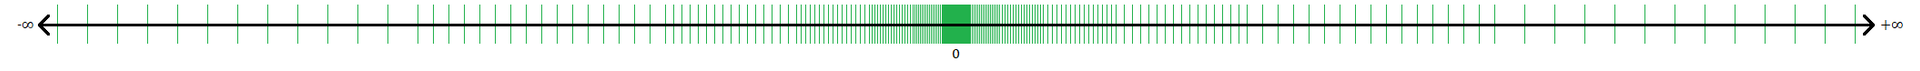
\includegraphics[width=\linewidth]{./figures/scaling.png}
          \caption{Verteilung von Gleitkommazahlen}
        \end{figure}
        \vspace{-0.5cm}
        \tiny
        \begin{table}
          \centering
          \begin{tblr}{
              cells = {c, white},
              column{1} = {PrimaryColor,fg=white},
            }
            $d[i]$      & 0.101 & 1.01 & 10.1 & 101 \\
            $\langle d[i]\rangle$  & 0.625  & 1.25 & 2.5 & 5 & \\
            $\langle d[i]\rangle - \langle d[i-1]\rangle$  & 0.3125 & 0.625 & 1.25 & 2.5 & \\
          \end{tblr}
          \caption{Abstände erhöhen sich exponentiel}
        \end{table}
      \end{itemize}
      \vspace{-1cm}
    \end{Sidenote}
  \end{itemize}
\end{frame}
\begin{frame}[allowframebreaks]{Appendix}{Hexadezimalsystem zu Binärsystem}
  \begin{align*}
    ba_{16} &= b_{16} \cdot 16^1 + a_{16} \cdot 16^0\\
            &= 13_{8} \cdot 16^1 + 12_{8} \cdot 16^0\\
      &= (1_{8} \cdot 8^1 + 3_{8}) \cdot 16^1 + (1_{8} \cdot 8^1+  2_{8}) \cdot 16^0\\
      &= (1_{8} \cdot 8^1 + 3_{8}) \cdot (8 \cdot 2)^1 + (1_{8} \cdot 8^1+  2_{8}) \cdot (8 \cdot 2)^0\\
      &= 2_{8} \cdot 8^2 + 6_{8} \cdot 8^1 + 1_{8} \cdot 8^1 \cdot (8 \cdot 2)^0 + 2_{8} \cdot (8 \cdot 2)^0\\
      &= 2_{8} \cdot 8^2 + 7_{8} \cdot 8^1 + 2_{8} \cdot 1 = 272_{8} \\
      ba_{16} &= b_{16} \cdot 16^1 + a_{16} \cdot 16^0\\
              &= 1011_{2} \cdot (2^4)^1 + 1010_{2} \cdot (2^4)^0 = 10111010_{2}
  \end{align*}
\end{frame}

% - sowohl um wegen keine zweiten 0 die 0 zu überspringen und direkt zu größten negativen Zahl zu springen, aber kann man es sehen, weil jetzt der kleinste Wert $-2^n$ ist und der größte Wert $2^n-1$
